%++++++++++++++++++++++++++++++++++++++++
% Don't modify this section unless you know what you're doing!
\documentclass[letterpaper,11pt]{article}
\usepackage{tabularx} % extra features for tabular environment
\usepackage{amsmath}  % improve math presentation
\usepackage{graphicx} % takes care of graphic including machinery
\usepackage[margin=1.3in,letterpaper]{geometry} % decreases margins
\usepackage{cite} % takes care of citations
\usepackage[final]{hyperref} % adds hyper links inside the generated pdf file
\usepackage{titlesec}
\usepackage{verbatim}
\usepackage{ragged2e}
\usepackage{amssymb}
\usepackage{tikz}
\usetikzlibrary{calc}
\tikzset{axis line style/.style={thin, gray, -stealth}}
\newcommand*{\TickSize}{2pt}
\setcounter{secnumdepth}{3}
\newtheorem{theorem}{Theorem}[section]
\newtheorem{property}{Property}[theorem]
\newtheorem{lemma}{Lemma}[theorem]

\makeatletter
\def\BState{\State\hskip-\ALG@thistlm}
\makeatother
\hypersetup{
	colorlinks=true,       % false: boxed links; true: colored links
	linkcolor=blue,        % color of internal links
	citecolor=blue,        % color of links to bibliography
	filecolor=magenta,     % color of file links
	urlcolor=blue
}
\newcommand\given[1][]{\:#1\vert\:}
\usepackage{listings}
\usepackage{array}
\usepackage{diagbox}
\usepackage{multicol}
\lstset{
  basicstyle=\ttfamily,
  mathescape
}
\usepackage{caption}
\usepackage{hyperref}

\usepackage{fvextra} % loads also fancyvrb
\usepackage{xpatch}

\DeclareMathVersion{ttmath}
\DeclareSymbolFont{latinletters}{OT1}{\ttdefault}{m}{n}
%\SetSymbolFont{latinletters}{ttmath}{OT1}{\ttdefault}{m}{n}
\SetSymbolFont{letters}{ttmath}{OML}{ccm}{m}{it}
\SetSymbolFont{symbols}{ttmath}{OMS}{ccsy}{m}{n}
\SetSymbolFont{largesymbols}{ttmath}{OMX}{ccex}{m}{n}

\newcommand{\changeletters}{%
  \count255=`A
  \advance\count255 -1
  \loop\ifnum\count255<`Z
    \advance\count255 1
    \mathcode\count255=\numexpr\number\symlatinletters*256+\count255\relax
  \repeat
  \count255=`a
  \advance\count255 -1
  \loop\ifnum\count255<`z
    \advance\count255 1
    \mathcode\count255=\numexpr\number\symlatinletters*256+\count255\relax
  \repeat
  \count255=`0
  \advance\count255 -1
  \loop\ifnum\count255<`9
    \advance\count255 1
    \mathcode\count255=\numexpr\number\symlatinletters*256+\count255\relax
  \repeat
}

\xapptocmd{\ttfamily}{\mathversion{ttmath}\changeletters}{}{}
%++++++++++++++++++++++++++++++++++++++++


\begin{document}

\title{\textbf{Practical Network Defense}\\ \bigskip \large Fourth Assignment - University ``La Sapienza"}
\date{2020-23-06}
\author{\textbf{Group 27}: Nicola Bartoloni ******* - Valerio Trenta 1856471}
\maketitle

\section{Scope and Initial Considerations}
The scope of this assignment is to setup a \textbf{Virtual Private Network} through \textbf{OpenVPN} in \textbf{OPNSense} to allow three authenticated \textit{Road Warriors} to access the internal subnetworks of \textbf{ACME Co.}, and to grant the usage of a \textbf{proxy server} on machine located at \textbf{100.100.6.3} -  which corresponds to domain \textbf{proxy.acme.group27} to the very same authenticated internal clients of the network to reach the \textbf{WAN} outside the \textbf{Main Firewall}.\\
Since these tasks are going to allow connections from the outside - even if authenticated and thus probably secured - it is a good idea to make sure, as a first step, that every user on each of the internal machines is protected by a strong password, and we will probably also have to confirm that the SSH protocol on each machine behaves as we expect it to behave - some of the \textit{root} accounts are already disabled by SSH on some machines, but some are still accepting connections based on basic authentication.\\
The next paragraphs will only deal with the two services we want to setup in the target network - \textbf{VPN} and \textbf{proxy server}.

\newpage
\section{Intrusion Prevention Systems setup}
It is explicitly required in the assignment to actually set up \textbf{Intrusion Prevention Systems}, so that they can not only detect intruders raising an alarm, but also perform actions in order to prevent the intrusion, like dropping suspicious packets. We are going to set up two different systems: in the two firewalls, we exploit the \textbf{suricata} service provided by the \textbf{OPNSense} administration panel to build a \textbf{Network Intrusion Prevention System}, while in the two hosts of the \textbf{DMZ subnetwork}, we download and configure the \textbf{fail2ban} tool to build a \textbf{Host Intrusion Prevention System}.\\
The differences and analogies between the two systems will be clear in the next two subparagraphs, as well as their configurations and functionalities.\\

\subsection{suricata}
The \textbf{suricata} service can be enabled in the \textbf{OPNSense} administration panel by navigating to \textit{System -$>$ Services -$>$ Intrusion Detection -$>$ Administration}. For both routers, we enable the service and we also check the box \textbf{IPS} to make it possible for the service to actually \textit{drop packets} matching a rule, so that it will not only raise an alarm, but also perform some concrete action in preventing the intrusion.\\
For both of them we also enable the \textbf{promiscuous mode} so that the systems will also monitor and check the rules for packets that are not strictly directed to one of their interfaces - so, obviously, forward packets will also be checked - and the \textbf{logging} service.\\
In the \textbf{Main Router}, we enable the service for \textit{all the interfaces, but the WAN interface}. This latter interface indeed is probably the one seeing the most of the traffic, being connected to the Internet, so we decide to run the system only at the interfaces directly connected to our services, so that when packets get there they have already been checked against the WAN interface's firewall rules and the interface itself won't be a bottleneck to the whole network just by checking every packet to every single rule of the \textbf{NIPS}.\\
In the \textbf{Internal Router}, the very same logic is applied and thus the service is only enabled on the \textbf{CLIENTS} and \textbf{SERVERS} interfaces.\\
Both systems in both firewalls are configured to update their rules daily according to a given schedule. Both of them will drop packets matching against one of the rules that have been selected.\\
The rulesets that are enabled follow below - and they are almost the same for both to apply defense-in-depth for the most internal firewall:\\

\begin{itemize}
\item all the rulesets from \textbf{Abuse.ch}, except \textit{Feodo Tracker}. These rules should detect compromised websites distributing malware, compromised and bad SSL certificates and such;
\item \textbf{ETOpen Attack-Response} catching common results of successful attacks;
\item \textbf{ETOpen botcc} for detecting Botnets and C2 hosts;
\item \textbf{ETOpen DOS} rules for DoS attacks;
\item \textbf{ETOpen DROP} rules for spam activities;
\item \textbf{ETOpen Exploit} and \textbf{ETOpen Malware} for detecting general exploits and malwares;
\item \textbf{ETOpen Inappropriate} rules for detecting accesses to inappropriate websites;
\item \textbf{ETOpen Policy} rules containing checks for things that are usually not enabled by a company policy - that seemed our case;
\item \textbf{ETOpen Scan} rules to prevent network scans, probes and in general reconnaissance activities;
\item \textbf{ETOpen Web rules} - \textit{client} in the Internal firewall, \textit{client and server} at the Main firewall, for web application security and prevention of common attacks - such as SQL injection, XSS;
\item finally, we also included some rules from the \textbf{OPNSense Suricata Application Detection}, namely for \textbf{file$-$transfer} and \textbf{mailing} applications - once again, it seemed our case to include these rulesets given the network belongs to a company, and clients are likely to be exploiting such applications.
\end{itemize}

The two routers do not seem to be overloaded by the rulesets that were applied, even if they are quite a lot and some might also be unnecessary - \textbf{botcc} and maybe the \textbf{Inappropriate} rules, the latter especially given the proxy and DNS service we set up previously.\\

\subsection{fail2ban}
The \textbf{fail2ban} tool can be downloaded on both the two machines running in the \textbf{DMZ}, namely the \textbf{proxy machine} and the \textbf{web machine}. We have three different services running on these machines, whose access we want to protect with this tool:

\begin{itemize}
\item \textbf{SSH} service running on both;
\item \textbf{apache2} service running on the \textbf{web machine};
\item \textbf{squid} service running on the \textbf{proxy machine};
\end{itemize}

so we copy the content of file \textit{$/$etc$/$fail2ban$/$jail.conf} in a new file, \textit{jail.local} under the same directory, which will be now used by \textbf{fail2ban} as configuration file for its jail. We leave unmodified the preconfigured values for parameters such as \textit{bantime} and \textit{maxretry} - 3600 and 5 - and we do not specify in neither of the two configurations for the two machines IP addresses that we want to ignore in the field \textit{ignoreip}, apart from the local loop, so that especially in the case of the \textbf{squid} service, we will monitor also accesses coming from the Clients subnetwork, so to prevent possible physical intrusions on the machines of the aforementioned subnet which may then lead to a misuse of the proxy service. The tool will then monitor the log files of the \textit{enabled} services in the \textit{jail.local} file to detect possible violations of authentication on those services - e.g., brute force attacks - and \textbf{ban} the hosts which made a number of attempts to authenticate that is $>$ \textit{maxretry}. To each services that we wish to monitor through the tool, we add the string \textit{enabled = true}. These services are:\\

\begin{itemize}
\item \textbf{sshd} in both the machines;
\item \textbf{apache2} and related lines in the \textit{jail.local} file for the \textbf{web machine};
\item \textbf{squid} for the \textbf{proxy machine}.
\end{itemize}

We enable and restart the \textbf{fail2ban service} through command line \textit{service fail2ban restart}. To check the list of jailed hosts per each service, we can execute command \textit{fail2ban-client status $<$service$>$}, as pictured in the figures below.\\

\begin{figure}[!htb]
\centering
\begin{minipage}{.5\textwidth}
  \centering
  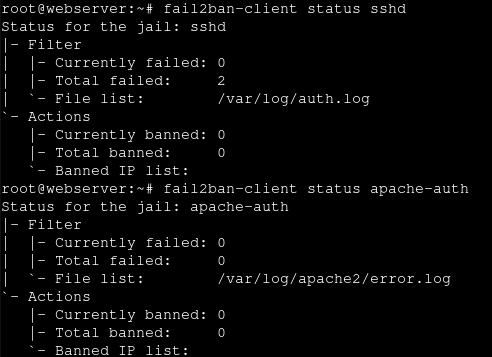
\includegraphics[width=1\textwidth]{fail2banWeb.png}
  \caption[a]{fail2ban jails for services in the Web machine (apache-auth is just one of the several apache jails we enabled).}\label{fig:7}
\end{minipage}%
\begin{minipage}{.5\textwidth}
  \centering
  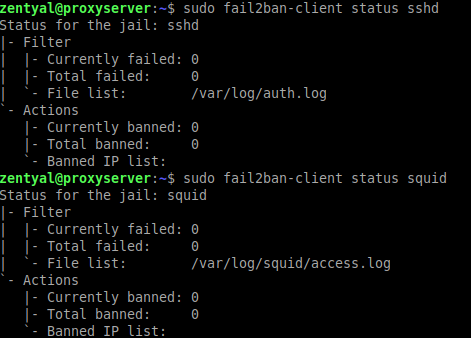
\includegraphics[width=1\textwidth]{fail2banProxy.png}
  \caption[a]{fail2ban jails for services in the Proxy machine.}\label{fig:7}
\end{minipage}%
\end{figure}

Please keep also in mind that we know that at least one more process is running on both machines - the \textbf{rsyslog} process for remote logging at log machine in the Internal servers - but this does not require any authentication mechanism so it is not monitored by the tool.

\newpage
\section{Engaging the Assessment}
In this section we are going to define the \textbf{scope} of the assessment, as weel as the typology of assessment we are going to carry out - i.e., which subnetworks we are going to test, and how prepared these subnetworks should be. Since we want to base our test upon the voices we heard in the company, if there is a new platform that is being developed, it is very likely to be placed in the \textbf{DMZ subnet}: indeed, it is likely that a platform belonging to our company is going to accept connections from visitors or external partners, and the \textbf{DMZ} is where this should happen.\\
Furthermore, our platform is surely going to exploit the services provided by our \textbf{Internal servers} - i.e. the logging service and the DNS service. This is why we should focus our assessment on these two subnetworks, so \textbf{DMZ} and \textbf{Internal servers} are going to be the subnetworks which define the perimeter of our assessment, our scope.\\
While the operations of \textbf{Linux hardening} we performed previously should not be rolled back during this assessment, we should ask ourselves how the other security measures we implemented are going to affect the tests als with respect of the typology of assessment we want to make. In order to gather as much information as possible about these two subnetworks, indeed, we should carry out the assessment with almost every security measure in the targets disabled. This is also due to the fact that the \textbf{GSM} machine is actually inside one of our target subnetworks (\textbf{Internal servers}), and while for the hosts in this subnet security measures such as firewalls or IPS are not going to affect the scan - traffic between scanning machine and targets is not going through any firewall at all - these measures could actually affect the scanning procedure of hosts in the \textbf{DMZ} subnet: indeed, we tried and found out that, with the firewall rules enabled, \textbf{GSM} is not able to perform the scan. This means that, to actually be able to find vulnerabilities in that subnetwork, we should at least get rid of the firewall - as if the \textbf{GSM} machine was in the same subnet. Obviously it is not, so the vulnerabilities that we are going to find out, have to be considered such in the worst case scenario - that is, an adversary who gained access to these two subnetworks and can send/receive Ethernet packets in there, for example gaining phyisical access to them or by performing some kind of spoofing attack.\\
The assessment results that we are going to describe and evaluate in the next section are, thus, obtained on the target hosts \textit{with firewalls and IPS (fail2ban and suricata) disabled}.

\newpage
\section{Vulnerability Assessment}
We are going to provide the results for each host on which the assessment was performed through \textbf{openVAS}, divided by subnet. We are going to adopt the \textbf{Severity Score} provided by \textbf{openVAS} for each of the vulnerabilities - on a scale from 0 to 10, each vulnerability is assigned a value that ranges in \textbf{None, Low, Medium, High} to describe its risk level. These values, along with their \textbf{Quality of Detection} score and the context, are then exploited to prioritize the most severe vulnerabilities in the \textbf{Analysis} subsection,where the vulnerabilities identified are discussed and mitigations are provided.\\
Every assessment was carried out requiring a minimum \textbf{QoD} of 70$\%$: we need to keep this in mind, since this minimum value, when met, means that the remote detection performed is not fully reliable.\\
Also, please notice that we are omitting several other information that \textbf{openVas} classified with severity score \textbf{Log} - 0.0. The only purpose of these information is to point out the results of different tests carried out by the tool that do not highlight vulnerabities by themselves, but are useful in the whole process and to us, as analyst, to check how the \textit{discovery, port scan, service detection and OS detection} phases were carried out by \textbf{openVAS}: some examples of these activities may be the execution of the \textbf{traceroute} command, \textbf{OS fingerprinting} operations, the \textbf{Services} log which points out all the services that were detected on the machine, \textbf{SSH} detection with corresponding algorithms to perform \textbf{encryption} and scans to determine which \textbf{cryptographic protocols} are exploited on the machine to perform \textbf{SSL/TLS}.\\
For each machine, the vulnerabilities to prioritize are highlighted in \textbf{bold}.

\subsection{Results}
\subsubsection{Internal Servers}
\textbf{DC machine - 100.100.1.2}
\begin{itemize}
\item \textbf{SSL/TLS Missing Secure Cookie Attribute - Severity Score: Medium};
\item \textbf{Missing httpOnly Cookie Attribute - Severity Score: Medium};
\item \textbf{SSL/TLS Certificate Signed Using A Weak Signature Algorithm - Severity Score: Medium};
\item TCP Timestamps - Severity Score: Low;
\end{itemize}
\begin{figure}[!htb]
\centering
\begin{minipage}{.5\textwidth}
  \centering
  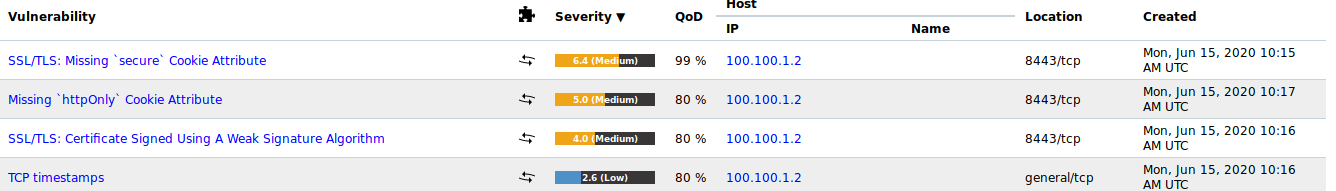
\includegraphics[width=1\textwidth]{dcVulns.png}
  \caption[a]{Vulnerabilities detected in the DC machine.}\label{fig:3}
\end{minipage}%
\end{figure}

\textbf{Log Server Machine - 100.100.1.3}
\begin{itemize}
\item TCP Timestamps - Severity Score: Low;
\end{itemize}
\begin{figure}[!htb]
\centering
\begin{minipage}{.5\textwidth}
  \centering
  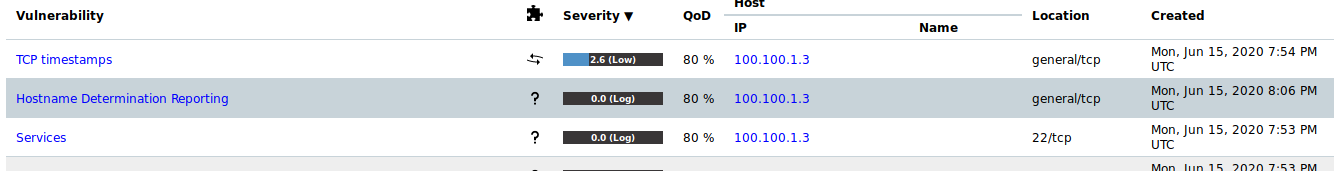
\includegraphics[width=1\textwidth]{logServerVulns.png}
  \caption[a]{Vulnerabilities detected in the Log Server machine.}\label{fig:4}
\end{minipage}%
\end{figure}

\textbf{GSM machine - 100.100.1.4}
\begin{itemize}
\item SSL/TLS: Untrusted Certificate Authorities - Severity Score: Medium;
\end{itemize}
\begin{figure}[!htb]
\centering
\begin{minipage}{.5\textwidth}
  \centering
  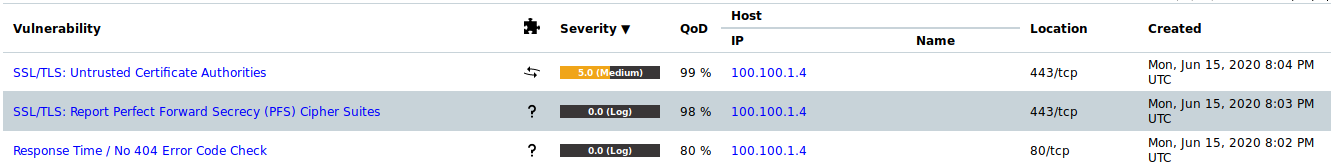
\includegraphics[width=1\textwidth]{GSM_vulns.png}
  \caption[a]{Vulnerabilities detected in the GSM machine.}\label{fig:5}
\end{minipage}%
\end{figure}

\subsubsection{Firewalls}
\textbf{Internal Firewall}
\begin{itemize}
\item \textbf{Cleartext Transmission of Sensitive Information via HTTP - Severity Score: Medium};
\item TCP timestamps - Severity Score: Low;
\end{itemize}
\begin{figure}[!htb]
\centering
\begin{minipage}{.5\textwidth}
  \centering
  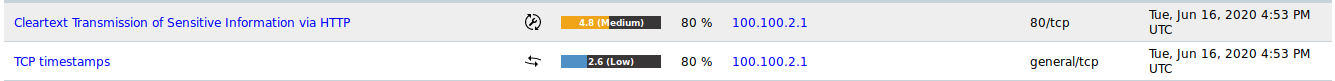
\includegraphics[width=1\textwidth]{internalFirewallVulns.png}
  \caption[a]{Vulnerabilities detected in the Internal Firewall machine.}\label{fig:6}
\end{minipage}%
\end{figure}

\textbf{Main Firewall}
\begin{itemize}
\item \textbf{Cleartext Transmission of Sensitive Information via HTTP - Severity Score: Medium};
\item TCP timestamps - Severity Score: Low;
\end{itemize}
\begin{figure}[!htb]
\centering
\begin{minipage}{.5\textwidth}
  \centering
  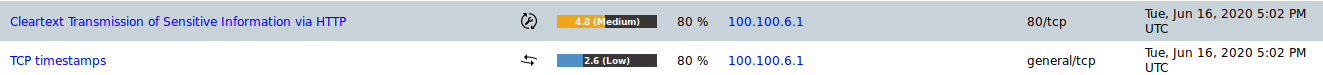
\includegraphics[width=1\textwidth]{mainFirewallVulns.png}
  \caption[a]{Vulnerabilities detected in the Main Firewall machine.}\label{fig:7}
\end{minipage}%
\end{figure}

\subsubsection{DMZ}
\textbf{Web Server Machine - 100.100.6.2}
\begin{itemize}
\item TCP timestamps - Severity Score: Low;
\end{itemize}
\begin{figure}[!htb]
\centering
\begin{minipage}{.5\textwidth}
  \centering
  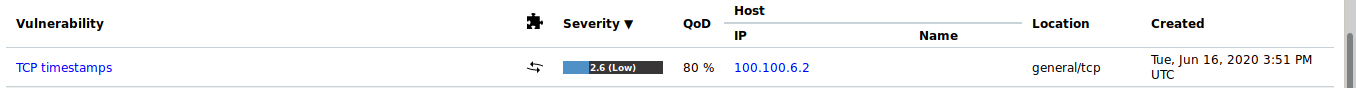
\includegraphics[width=1\textwidth]{webServerVulns.png}
  \caption[a]{Vulnerabilities detected in the Web Server machine.}\label{fig:8}
\end{minipage}%
\end{figure}

\textbf{Proxy Machine - 100.100.6.3}
\begin{itemize}
\item \textbf{SSL/TLS Missing Secure Cookie Attribute - Severity Score: Medium};
\item \textbf{Missing httpOnly Cookie Attribute - Severity Score: Medium};
\item \textbf{SSL/TLS Certificate Signed Using A Weak Signature Algorithm - Severity Score: Medium};
\item TCP Timestamps - Severity Score: Low;
\end{itemize}
\begin{figure}[!htb]
\centering
\begin{minipage}{.5\textwidth}
  \centering
  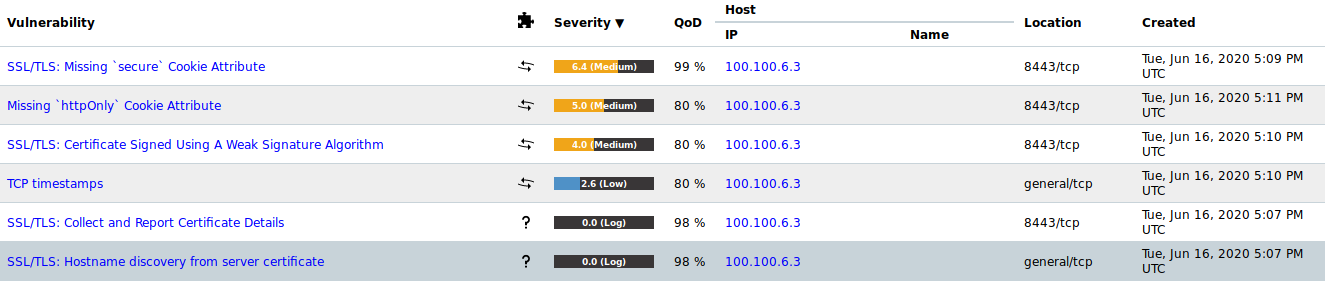
\includegraphics[width=1\textwidth]{proxyVulns.png}
  \caption[a]{Vulnerabilities detected in the Proxy machine.}\label{fig:9}
\end{minipage}%
\end{figure}

\subsection{Analysis}

Obviously, the fact that machines implementing the same services - \textbf{DC} and \textbf{Proxy} with \textbf{Zentyal}, both \textbf{firewalls} with \textbf{OPNSense} - were also diagnosed with the same vulnerabilities, is not simply due to chance. This is an advantage, since when we know how to fix a vulnerability in one of those machines, we also know how to fix it in the other one. We are thus now analyzing one by one the prioritized vulnerabilities - aslo explaining \textit{why} we chose to prioritize them - and then those that are left.\\

\subsubsection{Cleartext Transmission of Sensitive Information via HTTP}
\begin{itemize}
\item Severity Score: \textbf{Medium};
\item Affected Machines: Internal Firewall, Main Firewall (OPNSense);
\end{itemize}
\begin{figure}[!htb]
\centering
\begin{minipage}{.5\textwidth}
  \centering
  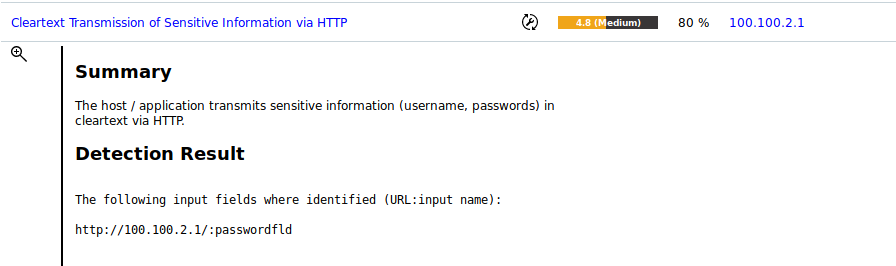
\includegraphics[width=1\textwidth]{clearTextHTTPfirewallVuln.png}
  \caption[a]{Password is sent in cleartext through HTTP.}\label{fig:10}
\end{minipage}%
\end{figure}

One of the desired features of a Firewall, is that of being immune to penetration. Firewalls are the first devices we should protect in our network, as they filter the traffic that is destined in/out from our subnetworks, and they also implement several other services (DHCP, suricata, OpenVPN...). Not to mention their importance in routing. This vulnerability affects the \textbf{OPNSense} service, and is due to the fact that \textbf{HTTPS} is not enabled.\\
This is probably the most important vulnerability to mitigate due to its potentially huge negative impact on our network and to the relatively easy fix.\\
Suggested way to mitigate this is indeed by checking at both firewalls the \textbf{HTTPS} box on option \textbf{Protocol} under \textit{System $->$ Settings $->$ Administration} as pictured in \textbf{Figure 11}: this way, authentication parameters - as well as any other data - should be sent through an encrypted channel. Since an adversary sniffing the devices' traffic might have already exploited this vulnerability, once mitigated it is also recommended to at least change all the passwords for each user in both firewalls.

\begin{figure}[!htb]
\centering
\begin{minipage}{.5\textwidth}
  \centering
  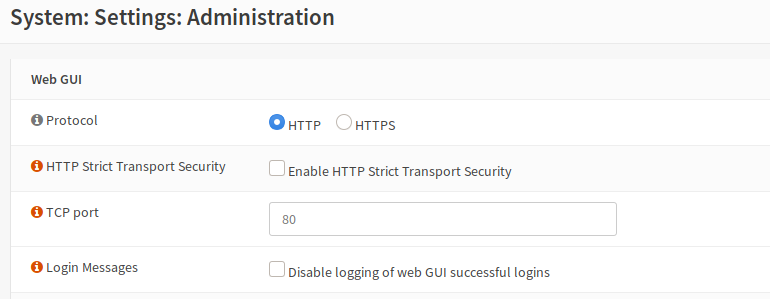
\includegraphics[width=1\textwidth]{vulnerabilityToMitigate.png}
  \caption[a]{Suggested fix.}\label{fig:11}
\end{minipage}%
\end{figure}

\subsubsection{SSL/TLS Certificate Signed Using A Weak Signature Algorithm}
\begin{itemize}
\item Severity Score: \textbf{Medium};
\item Affected Machines: DC, Proxy (Zentyal);
\end{itemize}
\begin{figure}[!htb]
\centering
\begin{minipage}{.5\textwidth}
  \centering
  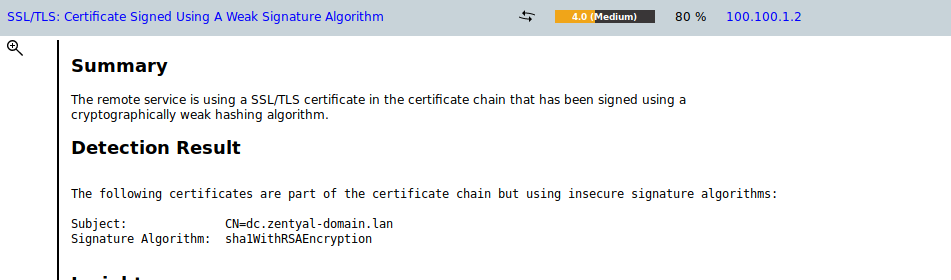
\includegraphics[width=1\textwidth]{weakSHA1CertificateDCVuln.png}
  \caption[a]{Certificate is signed with a weak algorithm - SHA1.}\label{fig:14}
\end{minipage}%
\end{figure}

The certificate provided for SSL/TLS sessions by both the machines is signed through \textbf{SHA-1 algorithm}, which is publicly known to be, nowadays, \textbf{not secure}, due to the fact that in 2017 the \textbf{Google Security Team} announced to have broken the algorithm by finding a collision. This means the certificate can be forged, it is possible to impersonate both machines and a \textit{MITM} attack is technically feasible on them. To mitigate this threat, it is recommended to generate a new certificate, one for each service running in the two machines, signed with a different algorithm, e.g. \textbf{SHA-250} or \textbf{SHA-3}. We do not know, though, whether this fix can be applied directly by us or it requires the vendor of the product.

\subsubsection{SSL/TLS Missing Secure Cookie Attribute}
\begin{itemize}
\item Severity Score: \textbf{Medium};
\item Affected Machines: DC, Proxy (Zentyal);
\end{itemize}
\begin{figure}[!htb]
\centering
\begin{minipage}{.5\textwidth}
  \centering
  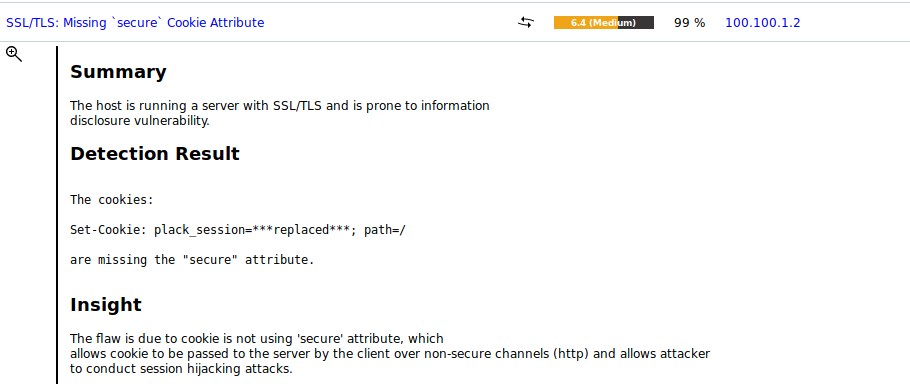
\includegraphics[width=1\textwidth]{secureCookiesDCVuln.png}
  \caption[a]{Cookies could be sent through an unencrypted channel.}\label{fig:12}
\end{minipage}%
\end{figure}

\textbf{Zentyal} service, reachable at port \textbf{8443} in both machines, already exploits the \textbf{HTTPS} protocol, so the server is running with \textbf{SSL/TLS}, but the \textit{Secure} flag is not sent for the cookies that may be used to remember an already authenticated user - meaning the cookies could be sent in clear text. This would allow an adversary which sniffs the traffic to read the cookie an authenticated client sends to the server, if the client sends it through an unencrypted channel, and exploit it to \textit{hijack his session} and be authenticated by \textbf{Zentyal} as an user with privileges, potentially leading to a disruption of the services running in the machines. We found no ways to actually instruct \textbf{Zentyal} on which cookies to accept and with which parameters - this might be a feature only available in the commercial edition, or only to the vendor of the product itself.\\
Beacuse of this, our only way to mitigate this vulnerability may be to make sure that no adversary is able to join the subnetworks of the two \textbf{Zentyal} machines and perform eavesdropping.

\subsubsection{Missing httpOnly Cookie Attribute}
\begin{itemize}
\item Severity Score: \textbf{Medium};
\item Affected Machines: DC, Proxy (Zentyal);
\end{itemize}
\begin{figure}[!htb]
\centering
\begin{minipage}{.5\textwidth}
  \centering
  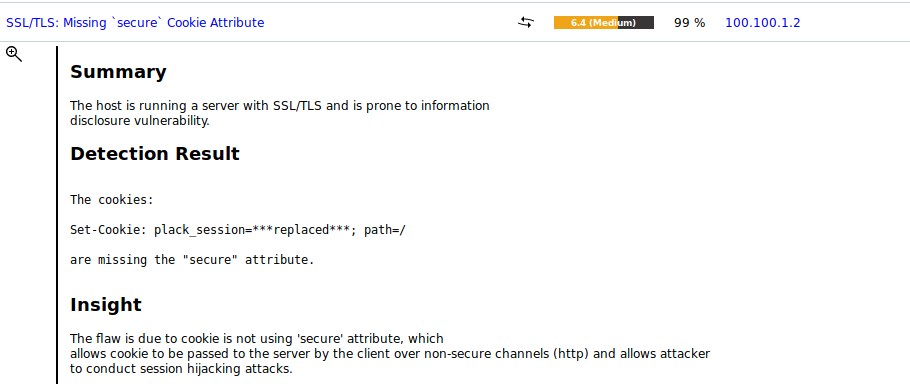
\includegraphics[width=1\textwidth]{secureCookiesDCVuln.png}
  \caption[a]{Cookies can be accessed through JavaScript code.}\label{fig:13}
\end{minipage}%
\end{figure}

This vulnerability is similar to the previous one, except it describes the cookies set by \textbf{Zentyal} to be missing the \textbf{httpOnly} attribute. This flag in a cookie prevents it from being accessed by scripts at client side - e.g. a JavaScript script accessing the cookie through the DOM of the web page. Just like the previous vulnerability, this might lead to \textit{session hijacking} as a result of \textit{XSS attacks}.\\
The only way to mitigate this vulnerability is the one we already highlighted in the previous subsection about \textbf{SSL/TLS Missing Secure Cookie Attribute} vulnerability.

\subsubsection{Low priority vulnerabilities}

\textbf{1. SSL/TLS: Untrusted Certificate Authorities}
\begin{itemize}
\item Severity Score: \textbf{Medium};
\item Affected Machines: GSM;
\end{itemize}
\begin{figure}[!htb]
\centering
\begin{minipage}{.5\textwidth}
  \centering
  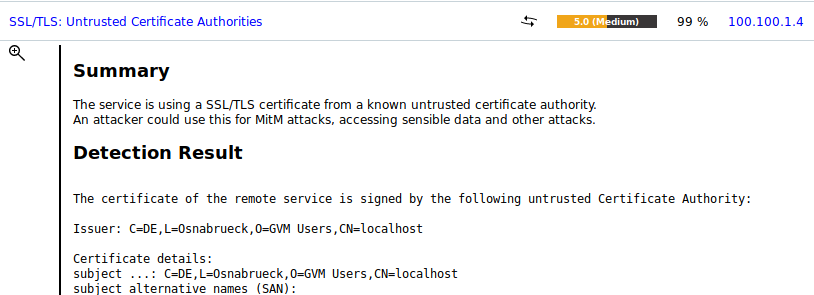
\includegraphics[width=1\textwidth]{certificateUntrustedAuthorityTLSGSM.png}
  \caption[a]{GSM - untrusted CA.}\label{fig:14}
\end{minipage}%
\end{figure}
This is probably a minor, false alarm: the CA signing the certificate for the \textit{GSM} machine is \textbf{Greenbone} itself, the scanner doesn't recognize it as a public, trustworthy CA, but we as users know it can be trusted.\\

\textbf{2. TCP timestamps}
\begin{itemize}
\item Severity Score: \textbf{Low};
\item Affected Machines: all, except GSM machine;
\end{itemize}
\begin{figure}[!htb]
\centering
\begin{minipage}{.5\textwidth}
  \centering
  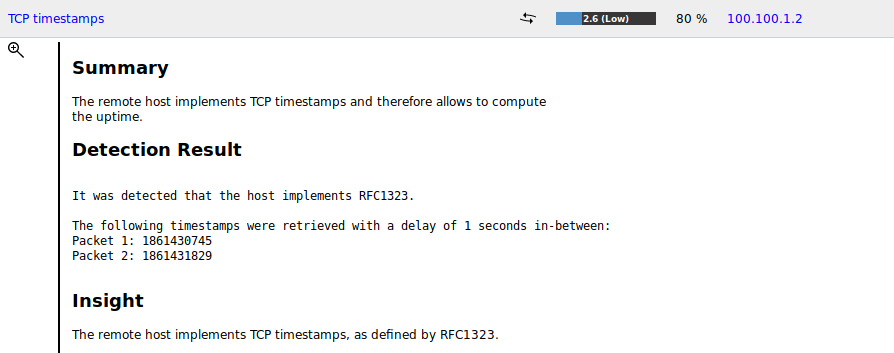
\includegraphics[width=1\textwidth]{tcpTimestampsVuln.png}
  \caption[a]{TCP Timestamps vulnerability in DC machine.}\label{fig:15}
\end{minipage}%
\end{figure}
\textbf{TCP timestamps} allow to compute the uptime of each host in the network. This provides extra information to an attacker, such as knowing when was the last time the machine was rebooted - which is something that occurs likely, for example, to install patches and updates. This might lead adversary to guess whether the system has installed the latest patches and updates, which might provide protection against latest exploits found on the system, or not, as well as to other exploits. However, hiding \textbf{TCP timestamps} for these reasons is basically \textit{security through obscurity}, which is commonly known to be a bad practice: real protection should be provided by always checking periodically the last updates and patches, and install them.\\
If needed, mitigation is provided by \textbf{openVAS} itself in the picture below, and can be easily applied to all the machines - but this might need further analysis, since disabling the TCP timestamps may also affect the system's performances as well as disable some other security features (see next section).\\
\begin{figure}[!htb]
\centering
\begin{minipage}{.7\textwidth}
  \centering
  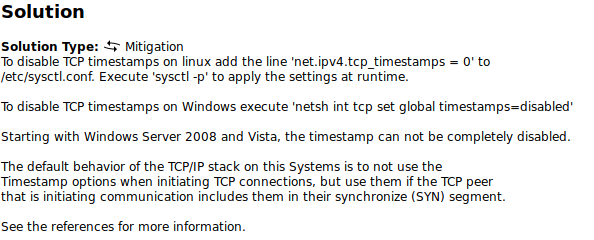
\includegraphics[width=1\textwidth]{tcpTimestampsVulnMitigation.png}
  \caption[a]{TCP Timestamps mitigation.}\label{fig:16}
\end{minipage}%
\end{figure}

\newpage
\section{Final remarks}
The testing phase showed us that the policy, if correctly interpreted, was implemented as specified by the assignment.\\
Some extra measures could have been taken, and they are very similar to the ones we have seen in the first assignment: we need to perform Linux hardening via sudo and hardening of the SSH protocol for all the machines in the DMZ and Internal Service subnetworks, and we need to change the default passwords for services such as \textbf{Zentyal} too and for users on the machines as well.\\
We should also stress the fact that, even if we found out that some of the machines had the SSH login via their \textit{root} account disabled by default, the scope of this assignment was to focus mainly on the \textbf{firewall rules} to be defined to achieve our goals and implement the given policy: this means that link$-$layer attacks were not taken into consideration, and this may be a critical vulnerability in our network. indeed, notice that every machine can be accessed through SSH or other protocols by any other machine on its same subnetwork - i.e., \textit{dc} can access \textit{logserver} through any protocol. This is because the rules we defined to implement our policy are placed on the two firewall$-$routers, which obviously do not handle packets exchanged between hosts in the same subnetwork: to overcome this issue, probably some extra rules should also be defined locally on each machine via \textit{iptables} - but this was out of our scope for this assignment.\\
We should also mention the fact that the \textbf{UDP} protocol was chosen to implement the \textbf{rsyslog} service, which could be also implemented through \textbf{TCP} protocol - commonly considered more secure - and maybe forced to exploit secure channels. Again, our goal here was to enable the service and enforce the policy via firewall rules, but we should stress the fact that just by exploiting TCP, this service may be hardened.\\
Also, as a last step, when the whole configuration going on in these assignments is over, we should at least enable only one machine in the \textbf{Clients} subnetwork - the \textbf{Kali} machine, probably - to connect via HTTP service to the two routers, for administration and practical reasons, so as we mentioned in the previous paragraphs, the rule enabling these connections should be actually disabled as a last step.

\newpage

\end{document}
